\chapter{Related Work}

\emph{Alternative title: Design Alternatives}\newline

\noindent
In this chapter important design alternatives for the R-tree and the LSM-tree are presented. The information gathered here is meant to be an introduction to how my implementation can be tuned to achieve a higher performance. 


\section{Packing R-trees}
The general packing method for R-trees was introduced in 1985\cite{DirectSpatialSearch}. In this method the rectangles in the dataset are sorted according to their center's x-coordinate. The rectangles are then packed into $k$ groups of $n$ rectangles each (except possibly the last one). Next, the MBR for each group is found and a pointer is set to the page that stores that group. Finally, the MBRs are packed recursively bottom-up in the manner explained above until the root node is created. 

\subsection{Sort-Tile-Recursive}
The Sort-Tile-Recursive (STR) method is a way of bulk-loading multi-dimensional data into R-trees and was introduced in 1997 by Leutenegger et al.\cite{STR}. For data with a dimension of $d=2$ the data is first sorted by their surrounding rectangle's x-coordinates. The x-coordinate is set to be the center for each rectangle. Further, STR uses a method called \emph{tiling} which divides the space into $S = \sqrt{r/M}$ vertical slices, where $r$ is the number of objects and $M$ is the maximum number of objects that fit in a node. Each slice has a certain amount of rectangles so that $\sqrt{r/M}$ nodes can be packed. The number of leaf nodes $P$ is set to $\lceil{r/M}\rceil$ as this gives the needed number of nodes to fit all the objects. Each slice is then filled with a partition of size $S \times M$ consecutive rectangles from the sorted list. It is important to notice that the last slice might contain fewer rectangles, as it is not guaranteed that the number of rectangles will fill the vertical slices fully. The last slice must however have a minimum of $m$ rectangles. Further, the rectangles for each slice are sorted internally by their y-coordinate and $M$ rectangles at a time are packed into nodes. To complete the tree, $M$ consecutive nodes are grouped together and put into a parent node. The last parent node might contain fewer than $M$ elements, but must have more than $m$. This is continued in a bottom-up manner until the root node is created. The Sort-Tile-Recursive method is also applicable for dimensions larger than two. \newline

\noindent
It has been shown that the STR method have performed better than other bulk-loading methods when the data is slightly skewed or have an uniform distribution. For highly skewed data, the performance gap between STR and the Hilbert packing method is quite similar\cite{STR}. The advantage with using the STR method is that in general there are less overlap between rectangles, which leads to fewer disk accesses as fewer elements of the tree needs to be searched. The difference in MBR overlap between the traditional R-tree, the improved R*-tree and the Sort-Tile-Recursive packed R-tree is shown in Figure \ref{fig:STRTree}.

\begin{figure}[ht]
    \centering
    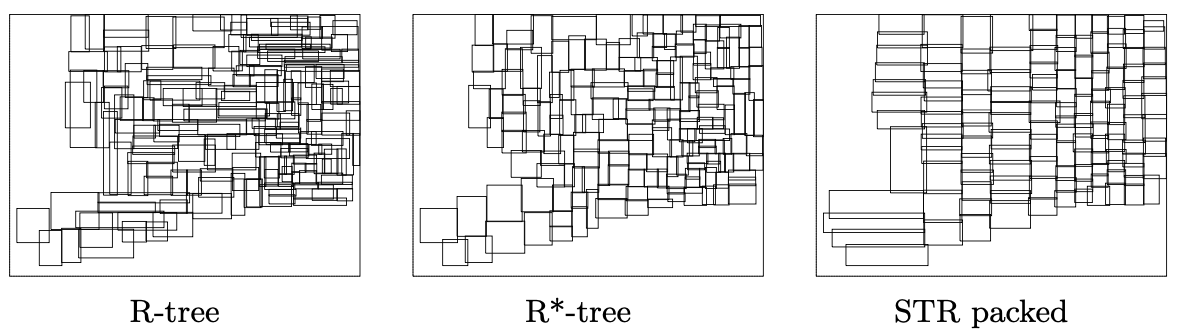
\includegraphics[scale=0.7]{figures/STR.png}
    \caption{MBRs of leaf nodes for R-tree, R*-tree and STR Packed R-tre\cite{RTreesTheoryApplications}}
    \label{fig:STRTree}
\end{figure}

\subsection{Small-Tree-Large-Tree Bulk-Insertion}
The Small-Tree-Large-Tree (STLT) bulk-insertion technique was presented in 1998 by L. Chen et al\cite{STLT} and is the first approach where bulk-insertion is used to update an existing R-tree, instead of creating an R-tree from scratch. Important aspects to conducting insertions into an existing R-tree is to make sure that the down-time is low so that queries can be conducted and that the query performance is not degraded to a large extent. In addition, it will reduce the insertion time as one does not have to build the entire R-tree from scratch with every insertion. To achieve bulk-insertion into an existing index structure, the STLT technique is designed for skewed data, i.e. data that are located in the same region. When new data is added, an R-tree index structure is created from it, which is called a small tree. A suitable location in the existing R-tree, also called the large tree, is found for insertion and the small tree is inserted here. By having skewed data, it can be ensured that the data inserted belongs to a certain location in the existing R-tree. In addition, down-time is reduced as only a small portion of the large tree is locked during the insertion.\newline

\noindent
The Small-Tree-Large-Tree method was also developed further in 1999 by introducing a Generalized Bulk-Insertion strategy (GBI)\cite{GBI}. GBI was introduced as the STLT technique only performs well with skewed data, while other distributions lead to overlapping MBRs which again have a degrading effect on the index structure and query performance. In the GBI approach, the data to be inserted is first clustered by using k-means. Small R-trees are then created from these clusters for a STLT insertion process. Outliers are inserted one by one. The advantage of GBI is that it is better suited for different types of data distributions, in addition to having query performance which is comparable to the traditional one-by-one approach proposed by Guttman\cite{r-tree}.

\subsection{Bulk-Insertion by Seeded Clustering}
Bulk-Insertion by Seeded Clustering was introduced by T. Lee et al in 2003 to maintain an efficient index structure for R-trees when bulk-insertion is utilized\cite{SeededClustering}. The general idea is to create input R-trees from clusters and inserting them into a single large, target R-tree. The seeded R-tree is first created from the top $k$ levels of the target R-tree, and this structure is used to classify data items into clusters. An input R-tree is then created from each of these clusters, which is shown to create less overlap between MBRs during bulk insertion. The insertion process is done by inserting the input trees into a node at height $h$ in the target R-tree. This height is equal to the height of the input R-tree, as this is required to maintain that all leaf nodes are at the same level. Another important part of the insertion is to make sure that the intermediate target node created during insertion does not suffer from node underflow, which is when the input root node contains fewer entries than $m$. To handle this issue, the entries of the root node of the input R-tree are reinserted into the target node. If the root node contains a number of entries higher than $m$, the input tree is directly inserted into the target node.\newline

\noindent
Finally, a repacking method is used if the root node from the input tree and the target node have many overlapping entries. This is done to maintain a good query performance. The method is done by repacking the overlapping entries from the target node with the input node. This is done in a bottom-up manner by first repacking the children and then repeating the process upwards. Bulk-insertion by seeded clustering has shown to outperform other bulk-insertion methods such as the Generalized Bulk-Insertion (GBI) with regard to both insertion and query performance. In addition, it has proven to have better query performance than R-trees with insertion one-by-one\cite{SeededClustering}.

\section{Merging R-trees}
Another approach to assemble R-trees was proposed in 2004 by Vasaitis, Nanopoulos and Bozanis\cite{MergingRtree}. Instead of using the bulk-insertion methods already in use, their method looks at merging two trees by taking advantage of the R-trees existing structure. It also does not make any assumptions about the data distribution which is the case in for example STLT, where the data is assumed to be skewed\cite{STLT}. The structure of the merging process consists of a splitting step similar to the one in R*-trees, tree insertion based on specific criteria and a merging algorithm. In order to merge two trees, the tree with the smallest height or the fewest elements are merged into the larger tree. The inserted tree is referred to as \emph{the giving tree}, while the tree inserted into is referred to as \emph{the receiving tree}. \newline

\noindent
To be able to perform the merge, two buffers of variable size are attached to every accessed node in the receiving tree. These are called \emph{insertion queue} and \emph{local insertion queue}. The insertion queue is used to store entries that are meant to be stored in the node itself and its child nodes. While the local insertion queue only stores entries that are meant to be stored in the node itself. In order to access these queues, additional external memory is needed compared to the traditional insertion method for R-trees. Only one page is needed to store the current node in the traditional insertion method, while $M+3$ pages are needed for the merging method. 2 pages for the insertion queue and 1 page for the local insertion queue in the node, and $M$ pages for the insertion queue in the child nodes.\newline

\noindent
The splitting method applied is similar to the one in R*-trees. The only difference is that when a split is conducted, the nodes where the entries are loaded into may also be full. To handle this, the split method is done in an iterative way to the children created from each split, until it is certain that all nodes contain at most $M$ entries. For the tree insertion, different criterias are used to decide if the giving tree's entries can be inserted as whole subtrees or if they need to be divided. This is done by looking at a) the area enlargement created by both the subtree and the sum of the individual entries, and inserting the option that gives the least area enlargement, or b) the overlap enlargement created in the current node by inserting the subtree and the individual entries, and inserting the option that gives the least overlap enlargement. The area criterion is used when the subtree is meant to be in a lower level of the receiving tree than the current one, while the overlap criterion is used when the subtree is meant to be in the current level.\newline

\noindent
The merging algorithm is executed by first picking the giving and receiving tree based on their sizes. Then the giving tree's root is inserted into the insertion queue of the receiving tree's root. Further, the tree insertion is executed and when a split occurs because of overflow, a new root is created for the receiving tree before the old root and the newly created nodes are inserted into its insertion queue. This is then done recursively until the merging process is finished. The merging of R-trees is shown to have a good query performance, and being able to execute the merging process efficiently\cite{MergingRtree}.

\section{Dynamic Hilbert R-trees}
The Hilbert R-tree was presented in 1993 by Ibrahim Kamel and Christos Faloutsos\cite{HilbertRTree}, and generates an R-tree where the rectangles have a linear ordering. When using a linear ordering, the goal is to keep similar objects close to each other. The selected ordering technique is the Hilbert curve, which is a space filling curve, shown to achieve the best clustering when compared to Z-order and Gray-code curve\cite{AnalysisHilbert}.\newline

\noindent
The best ordering found for the Hilbert R-tree was a method called \emph{2D-c}, which sorts the data rectangles based on the 2d-hilbert value of each rectangle's center. The node structure of the tree itself is similar to the general R-tree, where leaf nodes consists of (MBR, o). Non-leaf nodes contains an additional entry, known as the \emph{Largest Hilbert Value} (LHV), which gives the node structure (MBR, p, LHV). The largest hilbert value is the maximum hilbert value found in the MBRs enclosed by the non-leaf node's MBR. During insertions, the Hilbert R-tree uses a similar method as in B*-trees. In regular B-trees splitting a node is done when it overflows, and two nodes is created from the overflowed node. In B*-trees the splitting is delayed by trying to send entries to sibling nodes when the original node is overflowed. The number of siblings can be chosen as \emph{s}, and when all sibling nodes are full, the split will be conducted by creating \emph{s+1} nodes to handle the overflow entry. The best trade-off for choosing siblings is shown to be 3-to-4 splitting, which entails having three siblings. This gives the best insertion speed, which decrease with the increase of siblings, while maintaining a good performance, which increase with the number of siblings.\newline 

\noindent
In the original presentation of the Dynamic Hilbert R-tree it is shown that it outperforms R*-trees on response time by up to 28\%\cite{HilbertRTree}. It has however later been discovered that the Dynamic Hilbert R-tree is vulnerable to large objects performance-wise. In addition the proximity is not kept to a satisfying degree by the Hilbert curve as the space dimensionality increases, which leads to MBRs overlapping more in internal tree nodes\cite{RTreesTheoryApplications}.

\section{Dostoevsky}
\label{Dostoevsky}
An optimization of LSM-trees was introduced in 2018 by Niv Dayan and Stratos Idreos. Their research introduces a concept called \emph{Dostoevsky}, in full \emph{Space-Time Optimized Evolvable Scalable Key-Value store}\cite{Dostoevsky}. The solution consists of taking advantage of the different merge policies \emph{tiering} and \emph{leveling} to find the best trade-off between update costs and lookup costs. An important find in their research is that by only conducting merge operations on the largest level, the update cost is improved without affecting lookup or storage costs to an important extent. As updates in LSM-trees are executed by sending it down through the levels, old entries in the largest level are outdated and takes up unnecessary space. In addition, all entries will be merged in every level since outdated entries are not removed until its updated value reaches the largest level.\newline 

\noindent
To take advantage of these characteristics, a design solution called \emph{Lazy Leveling} is introduced. Lazy Leveling is designed so that only the largest level conducts any merge operations, while all levels above consists of a tiering merge policy. By having this implementation the cost of merging entries at each level is avoided, which in turn reduces the update cost. To be able to tune the design of the LSM-tree, Lazy Leveling is incorporated in another design solution called \emph{Fluid LSM-tree}. In this approach, the largest level is also separated from the smaller ones. This is done by assigning a maximum run size of $Z$ to the largest level, while a maximum run size of $K$ is given to the levels above. To accommodate these sizes, each level also have an \emph{active run} with a size threshold of $T/K$ or $T/Z$ for the smaller and largest levels respectively. $T$ is set to be the ratio between adjacent levels. When these active runs reaches their threshold, their runs are merged into the lower level's active run. The use of Lazy Leveling in the Fluid LSM-tree comes into effect when setting the parameters $K=T-1$ and $Z = 1$. If both parameters are set to $T-1$, the LSM-tree has a tiering merge policy. With parameters set to $1$, the merge policy chosen is leveling. \newline

\noindent
In order to tune the Fluid LSM-tree correctly according to the application area, the tuning parameters are set while having a constraint on space amplification. The goal is to optimize throughput by looking at update cost, zero-result point lookup cost, non-zero result point lookup cost and range lookup cost. Each of these values are weighted and multiplied by the time it takes to read a block from storage. In order to check the worst-case scenario, the different values are found by setting different parameters for $T$, $Z$ and $K$. The calculation is then iterated. The automatic way of finding the best settings for the parameters, as explained above, is called Dostoevsky. This solution is shown to have much better results than existing solutions such as RocksDB\cite{Dostoevsky}. This is due to the fact that RocksDB only uses leveling, while Dostoevsky is able to change the merge policy of its levels in-between workloads.